\documentclass[12pt, twoside]{article}
\usepackage{jmlda}
\newcommand{\hdir}{.}
\usepackage{natbib}
\usepackage[dvipdfm]{graphicx}
\begin{document}

\title
    [Поиск зависимостей в биомеханических системах] % краткое название; не нужно, если полное название влезает в~колонтитул
    {Поиск зависимостей в биомеханических системах}
\author
    [Зыков Т.А.] % список авторов (не более трех) для колонтитула; не нужен, если основной список влезает в колонтитул
    {Зыков~Т.А.} % основной список авторов, выводимый в оглавление
    [Зыков~Т.А.$^1$, Дорин~Д.Д.$^2$, Стрижов~В.В.$^{3}$] % список авторов, выводимый в заголовок; не нужен, если он не отличается от основного
\email
    {zykov.ta@phystech.edu}
\organization
    {$^1$Chair of Data analysis; $^2$, $^3$Intelligent systems;}
\abstract
    {% Данный текст является шаблоном статьи, подаваемой для публикации в журнале <<Машинное обучение и анализ данных>>.

    
   Исследуется проблема восстановления зависимости между показаниями датчиков фМРТ и восприятием внешнего мира человеком. Проводится анализ зависимости между последовательностью снимков фМРТ и звуковым рядом. Требуется предложить метод прогнозирования показаний фМРТ по прослушиваемому звуковому ряду. При прогнозировании сложноорганизованных временных рядов, зависящих от экзогенных факторов и имеющих множественную периодичность, связи между рядами устанавливаются с помощью теста Гренджера. 
}
\maketitle

\section{Введение}

Функциональная магнитно-резонансная томография (фМРТ)~\citep{puras2014neurovisualization} — метод нейровизуализации, который измеряет активность мозга путем выявления изменений, связанных с кровотоком. Метод нейровизуализации фМРТ находит применение для анализа корреляции активности мозга с такими заболеваниями как аутизм и болезнь Альцгеймера, а также для прогнозирования таких заболеваний как черепно-мозговая травма и имеет потенциал для терапии~\citep{fmriapplications}. Он дает представление о том, какие области мозга участвуют в конкретных психических процессах или задачах, измеряя уровень BOLD (Blood-oxygen-level-dependent). BOLD --- это показатель, используемый в функциональной магнитно-резонансной томографии, который отражает изменения кровотока и уровня насыщения кислородом в мозге~\citep{bold}. 

Работа посвящена восстановлению зависимости между снимками фМРТ
и звуковым рядом. Предполагается, что такая зависимость существует. Кроме того, предполагается, что между снимком и звуковым рядом есть постоянная задержка во
времени~\citep{menon1999spatial}. Время задержки выступает в качестве гиперпараметра модели. Предлагается метод аппроксимации показаний фМРТ по прослушиваемому звуковому ряду. Проводится первичный анализ влияния типа звукового ряда (музыка или простой диалог) на изменения уровня BOLD и анализ зависимости снимков фМРТ от звукового ряда.

В данной работе рассмотрим одно из ограничений BOLD~\citep{menon1999spatial}. Временное разрешение -- это наименьший период времени нейронной активности который с высокой точностью можно определить с помощью фМРТ. Время измерений фМРТ происходит с задержкой, что затрудняет регистрацию быстрых нейронных событий. Кроме того, при выборе модели важно учитывать структуру временных рядов: у некоторых вокселей прослеживается тренд на протяжении всей звуковой дорожки или неоднородность шума, при которых нужно использовать оценки Уайта~\citep{hetero}.

Для извлечения признаков из звуковой дорожки предлагается использовать разные подходы~\citep{audiofeaturetrends}. В этой работе рассматривается мел-кепстральные коэффициенты (MFCC). Это характеристики аудиосигнала которые получаются из спектрограммы и используются для анализа звука и обработки речи. Преимуществом такого представления является небольшая размерность.

В качестве выборки будем использовать данные~\citep{Berezutskaya2022}, собранные у большой группы людей во время просмотра короткометражного аудиовизуального фильма. Он включает записи фМРТ 30 участников в возрасте от 7 до 47 лет. Данные были получены с использованием богатого аудиовизуального стимула. Звуковая дорожка состоит из диалогов персонажей и музыкальных вставок.


\section{Постановка задачи}
Требуется предложить метод прогнозирования показаний фМРТ по прослушиваемому звуковому ряду. 
Обозначим частоту снимков фМРТ $\mu \in \mathbb{R}$. Задана последовательность снимков
\begin{equation}
	\label{eq1}
	\bS = [\bs_1, \ldots, \bs_{\mu t}], \quad\
	\bs_{\ell} \in \mathbb{R}^{X \times Y \times Z},
\end{equation}
где $X, Y$ и $Z$~--- размерности воксельного изображения.

Задана частота дискретизации $\nu \in \mathbb{R}$, количество каналов $k \in \mathbb{N}$ и продолжительность $t \in \mathbb{R}$ аудиоряда.
Задан непрерывный по времени сигнал
\begin{equation}
	\label{eq2}
	\bP = [\bp_1, \ldots, \bp_{\nu t}], \quad\
	\bp_{\ell} = 
        \begin{pmatrix}
        p_\ell^1\\
        p_\ell^2 \\
        \vdots \\
        p_\ell^k\\
        \end{pmatrix}, \quad\
	p_{\ell}^k \in \mathbb{R},
\end{equation}

Задача состоит в 
построении отображения, которое бы учитывало задержку $\Delta t$ между
снимком фМРТ и аудиорядом, а также предыдущие томографические показания. Формально, необходимо
найти такое отображение $\mathbf{f}$, что
\begin{equation}
	\label{eq3}
	\mathbf{f}(\bp_1, \ldots, \bp_{k_{\ell} - \nu \Delta t}; \bs_1, \ldots, \bs_{\ell-1}) = \bs_{\ell},
	\ \ell = 1, \ldots, \mu t,
\end{equation}
где для $\ell$-го снимка фМРТ номер соответствующего сигнала $k_{\ell}$ определяется по формуле
\begin{equation}
	\label{eq4}
	k_{\ell} = t\nu = \dfrac{\ell}{\mu}\nu.
\end{equation}

Эмбеддингами аудиоряда будут мел-кепстральные коэффициенты~\citep{mfcc}. То есть
для каждого экземпляра сигнала имеем вектор размерности $\mathbf{d}$:
\begin{equation}
	\label{eq5}
 \bx_{\ell} = [x^{\ell}_1, \ldots, x^{\ell}_{d}]\T \in \mathbb{R}^{d}, \ {\ell} = 1, \ldots, \dfrac{\nu t}{h}. 
\end{equation}
Будем восстаналивать функцию $\mathbf{f}$, в предположении марковского свойства. 

\begin{equation}
	\label{eq6}
	\mathbf{f}(\bx_{k_\ell - 
 \nu\Delta t - g}, \ldots, \bx_{k_\ell - 
 \nu\Delta t}) = \bs_\ell - \bs_{\ell-1} = \bdelta_\ell
	\ \ell = 2, \ldots, \mu t,
\end{equation}
где $\bdelta_{\ell} = [s^{\ell}_{ijk} - s^{\ell-1}_{ijk}] = [\delta^{\ell}_{ijk}] \in \mathbb{R}^{X \times Y \times Z}$~--- разность между двумя последовательными снимками.


Учитывая \eqref{eq4}, суммарное число пар (сигнал, снимок)
равно $N = \mu (t - \Delta t)$. Таким образом, для каждого вокселя задана выборка
\[ \mathfrak{D}_{ijk} = \{(\bx_{\ell}, \delta^{\ell}_{ijk}) \ | \ {\ell} = 2, \ldots, N \}. \]

Поставлена элементарная задача восстановления регрессии
\begin{equation}
	\label{eq7}
	y_{ijk}: \mathbb{R}^{d} \to \mathbb{R}.
\end{equation}

Рассмотрим каждый воксель независимо $\mathbf{Y}_{ijk} \in \mathbb{R}^{N}$ --- воксели, $\mathbf{X} \in \mathbb{R}^{N \times d}$. Предполагаемая зависимость
\begin{equation}
	\label{eq8}
	\mathbf{Y}_{ijk} = \mathbf{X}\mathbf{\theta} + \varepsilon,
\end{equation}
где $\mathbf{\theta} \in \mathbb{R}^d$ - коэффициенты модели, $\varepsilon \sim N(0, \Sigma)$ - шум.

Требуется найти параметры $\mathbf{\widehat\theta}$, доставляющие максимум функции правдоподобия при заданных гиперпараметрах $\Delta t$ и $d$, где $d$ -- размерность MFCC:
\begin{equation}
	\label{eq9}
	L_X(\theta) = \prod\limits_{v=1}^N p_\theta(Y_{ijk}^v) \longrightarrow \mylim{max}_\theta
\end{equation}

\section{Предварительные сведения}

Снимки фМРТ были отнормированы на отрезок [0, 1] c чисткой от некоторых выбросов. В качестве размерности MFCC взят $d = 15$. Общие характеристики обработанного датасета представлены в таблице~\ref{table:sample}.

В снимках фМРТ присутствуют воксели с неоднородным шумом и/или с линейным трендом.

Для большей информативности входа для предсказания следующего вокселя, вместо одного вектора MFCC подавалось усреднение по окну размера 50. Также добавлена константа (intercept) к данным.
\begin{figure}[h!]
	\centering{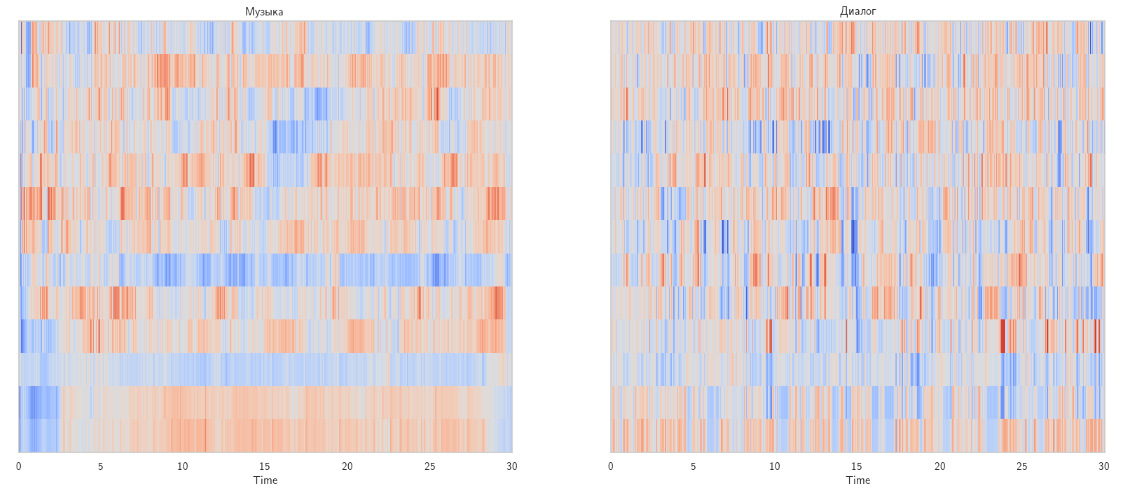
\includegraphics[width=1\textwidth]{mfcc_desc.eps}}
	\caption{Коэффициенты MFCC}
	\label{fig:example}
\end{figure}

\begin{table}[h!]
	\centering
	\caption{Описание датасета}
	\begin{tabular}{|c|c|c|}
		\hline
		Характеристика                       & Значение            \\
		\hline \hline
		длина короткометражного фильма         & 389 сек.                \\ \hline
		частота снимков фМРТ           & $641 / 389 \approx 1.65$ Гц   \\ \hline
		частота звукового ряда           & $\mu$ \\ \hline
		звуковой ряд       & $[-1, 1]^{2 \times 390 \times 44100}$         \\ \hline
		снимок фМРТ             & $[0, 1]^{40 \times 64 \times 64}$           \\ \hline
	\end{tabular}
	\label{table:sample}
\end{table}


\section{Вычислительный эксперимент}

Ниже приведен пример работы алгоритма на снимках седьмого испытуемого. Все срезы по 20-й координате.

\begin{figure}[h!]
	\centering{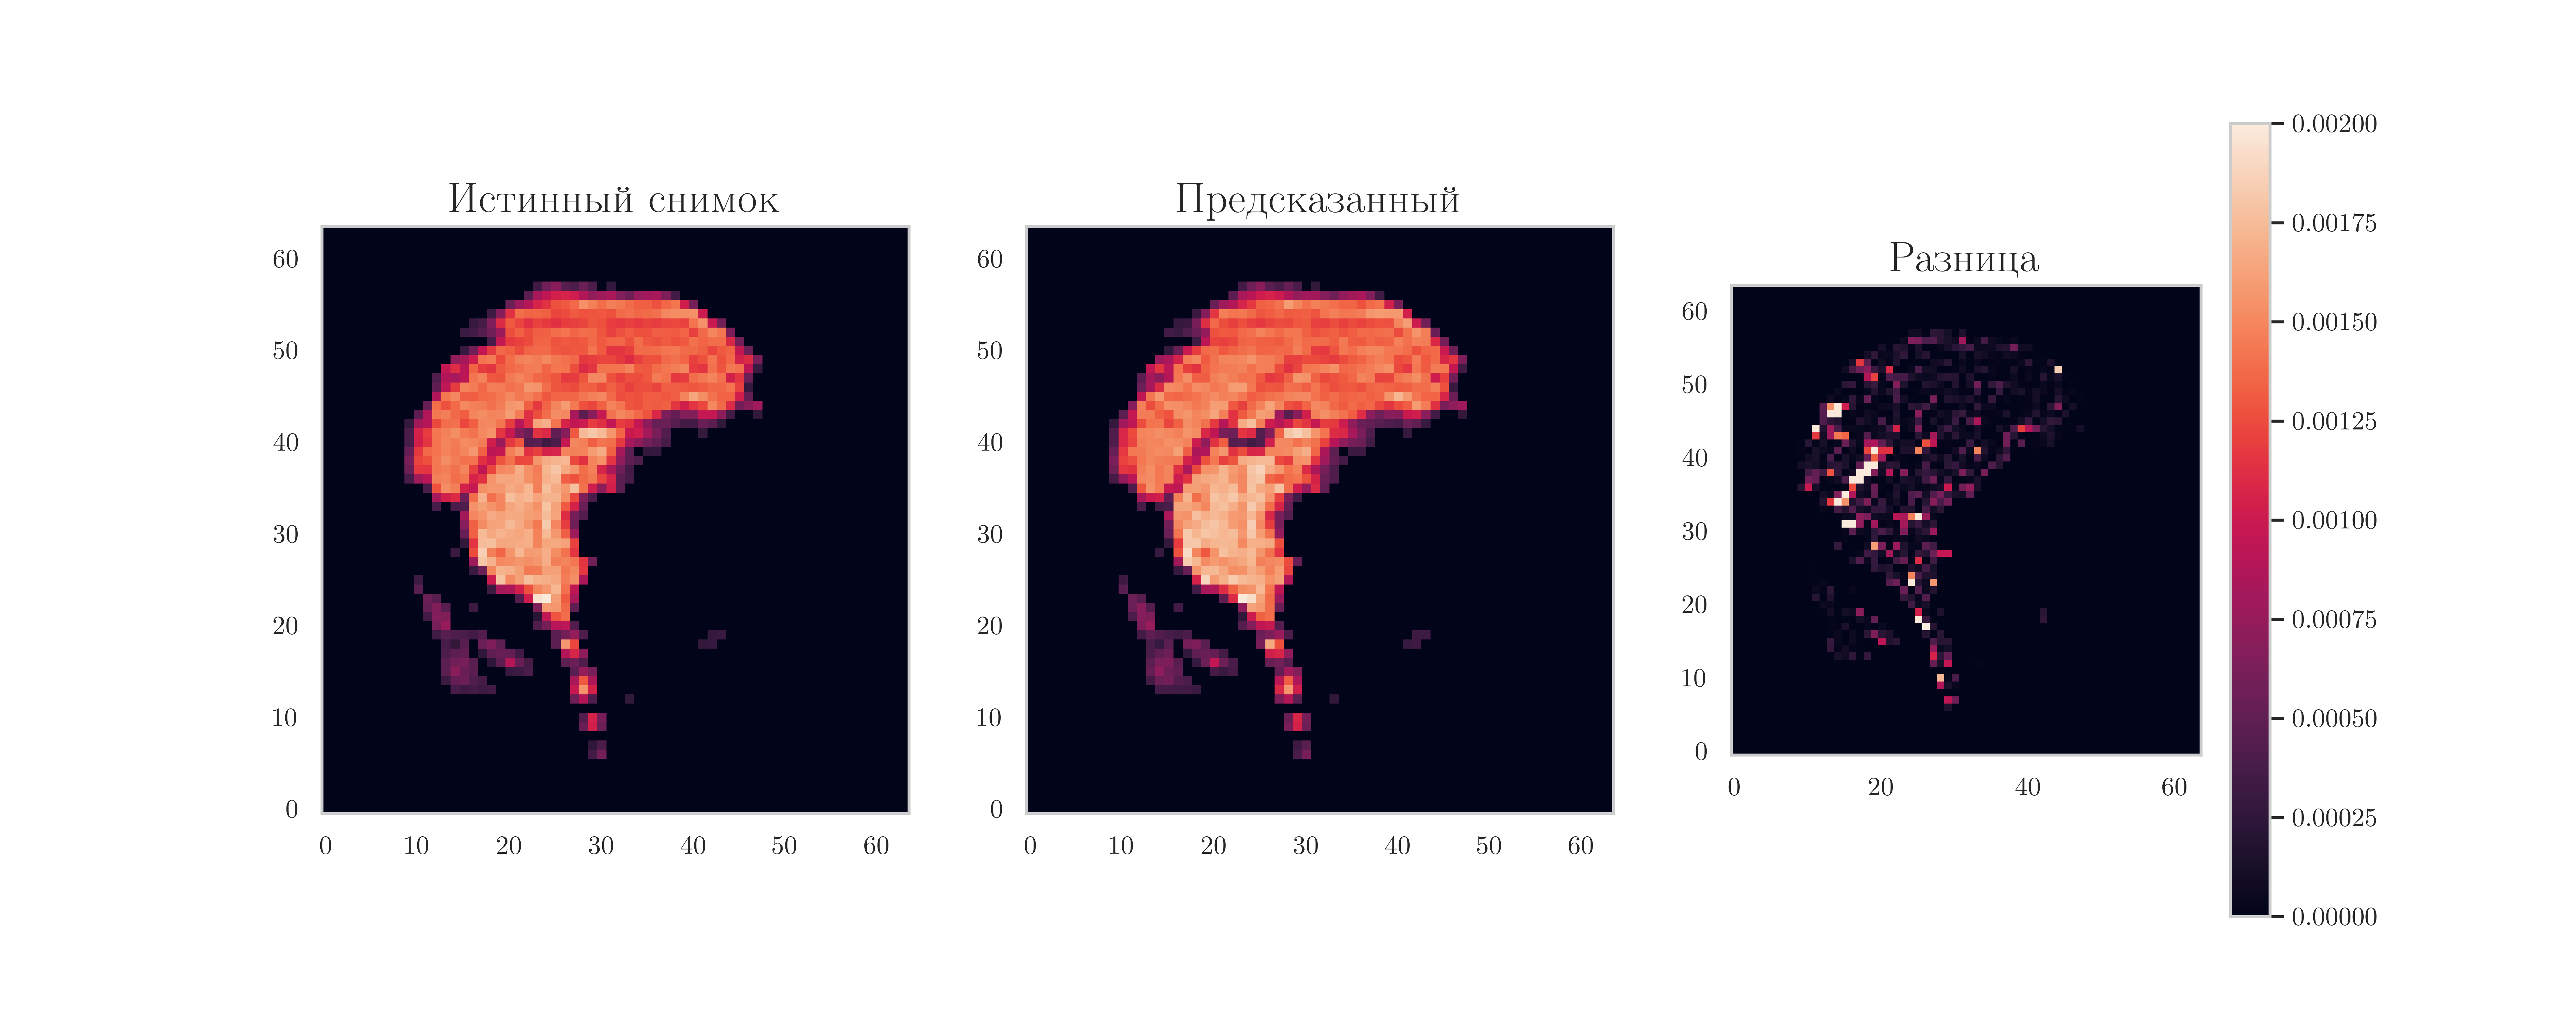
\includegraphics[width=1\textwidth]{example.png}}
	\caption{Пример работы алгоритма}
	\label{fig:example}
\end{figure}

Оценивать качество модели на предсказанных следующих по порядку снимках некорректно. Снимки отличаются на очень малую величину. Обучим вторую модель, одинаковую по архитектуре, на неинформативном входе (случайный тензор) и сравним его в рекурсивной стратегии предсказания.

\begin{figure}[h!]
	\centering{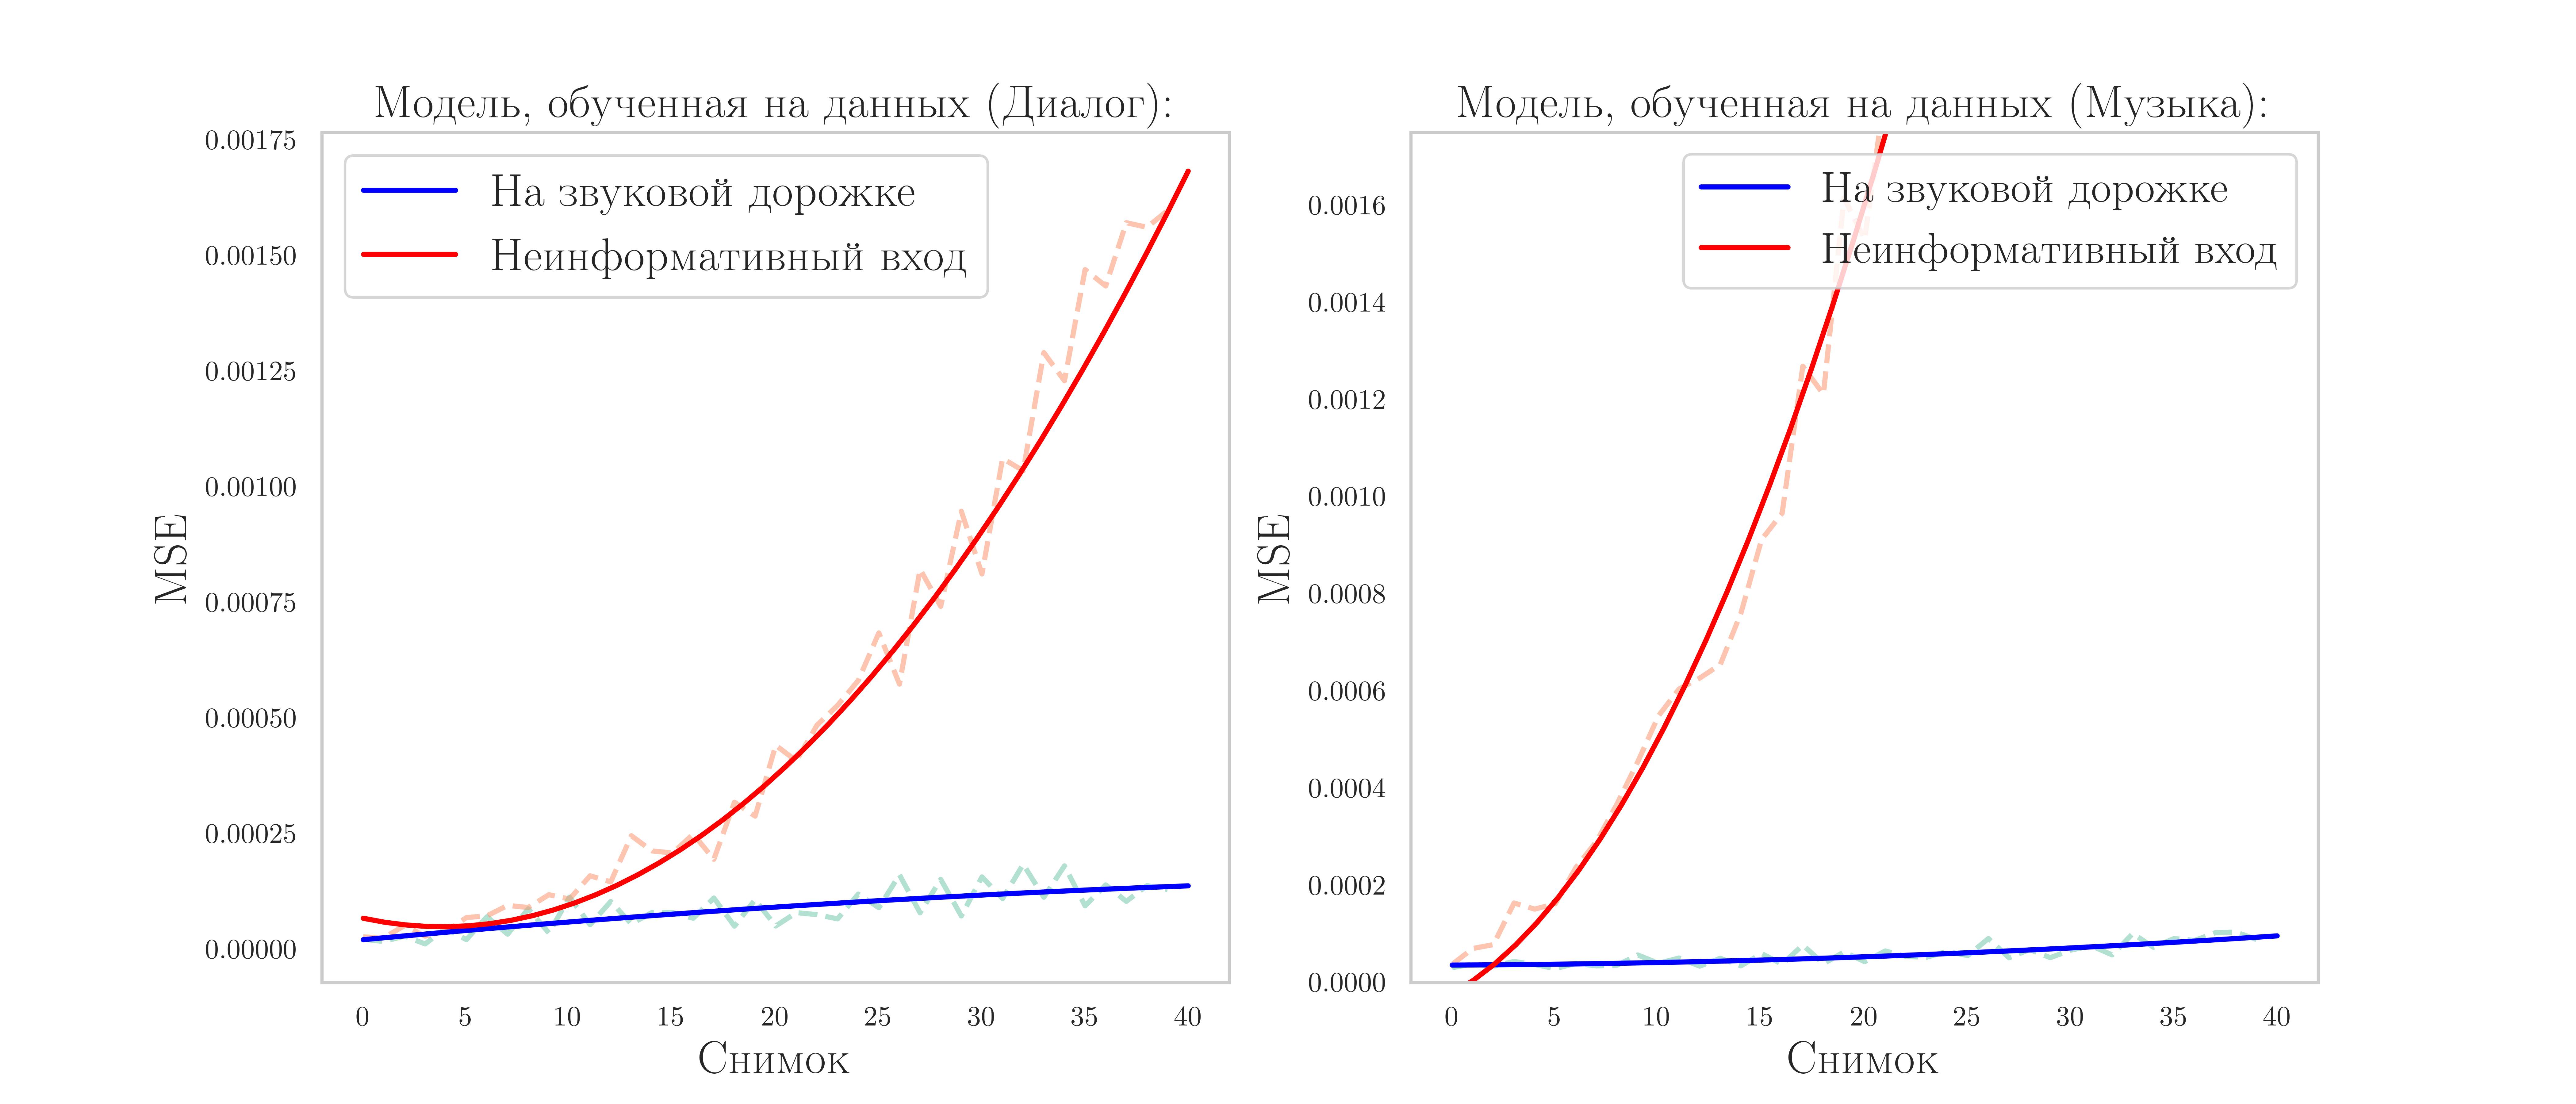
\includegraphics[width=1\textwidth]{recursive.png}}
	\caption{Сравнение MSE моделей}
	\label{fig:example}
\end{figure}

Заметим, что наша модель работает намного лучше и меньше накапливает ошибку. Следовательно, звуковая дорожка имеет свой эффект на изменение вокселей фМРТ.

Распределение весов модели, которое представлено в рис.~\ref{fig:weights}, невырождено. Это происходит из-за того, что ряды вокселей похожи на стационарные.

\begin{figure}[h!]
	\centering{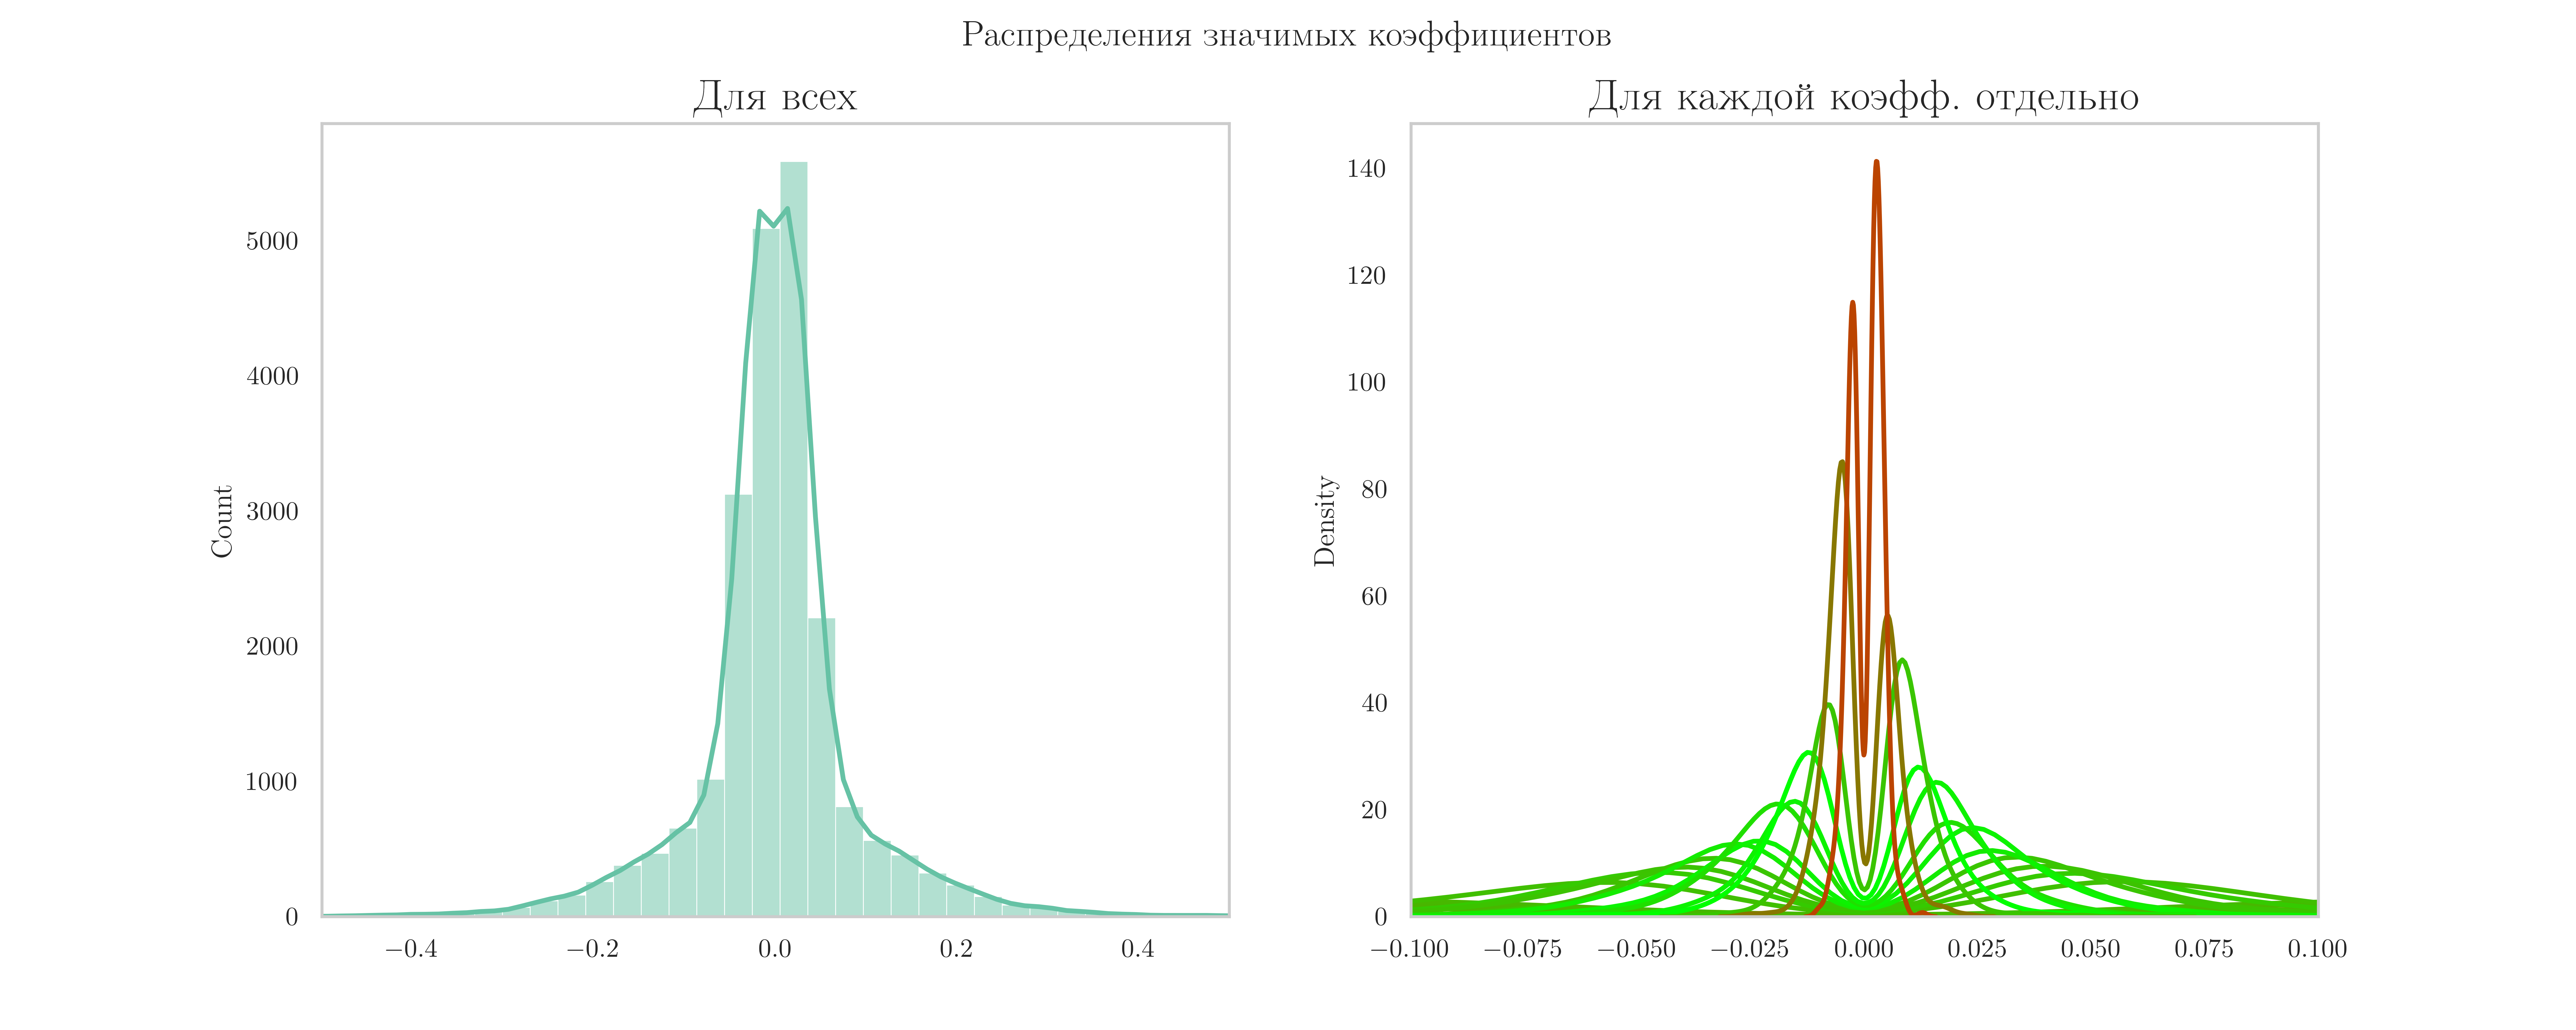
\includegraphics[width=1\textwidth]{model_weights_distribution.png}}
	\caption{Распределение весов}
	\label{fig:weights}
\end{figure}

\section{Анализ решения}

Очевидно, звук оказывает влияение не на все области мозга. Выделим воксели, на которые звуковой ряд влияет по Грэнджеру~\citep{granger}. Важно помнить, что причинность по Грэнджеру является необходимым, но не достаточным условием причинно-следственной связи.

Зафиксируем воксель $i$. Пусть $X$ -- временной ряд звуковых сигналов, $Y$ -- ряд значений вокселя $i$ на снимках фМРТ. Строится модель регрессии:

\begin{equation}
	\label{eq10}
	Y_{t}=a_{0}+a_{1}Y_{t-1}+...+a_{p}Y_{t-p}+b_{1}X_{t-1}+...+b_{p}X_{t-p}+\varepsilon _{t}
\end{equation}



Нулевая гипотеза заключается в том, что коэффициенты при лагах второй переменной одновременно равны нулю. Данную гипотезу предлагается проверить простым критерием Фишера~\citep{hetero}.

Рассмотрим пересечение вокселей, у которых pvalue меньше 0.3, и височных долей мозга, согласно исследованиям~\citep{brain}. Пример вокселя, у которого околонулевое pvalue на рис.~\ref{fig:voxel}.

\begin{figure}[h!]
	\centering{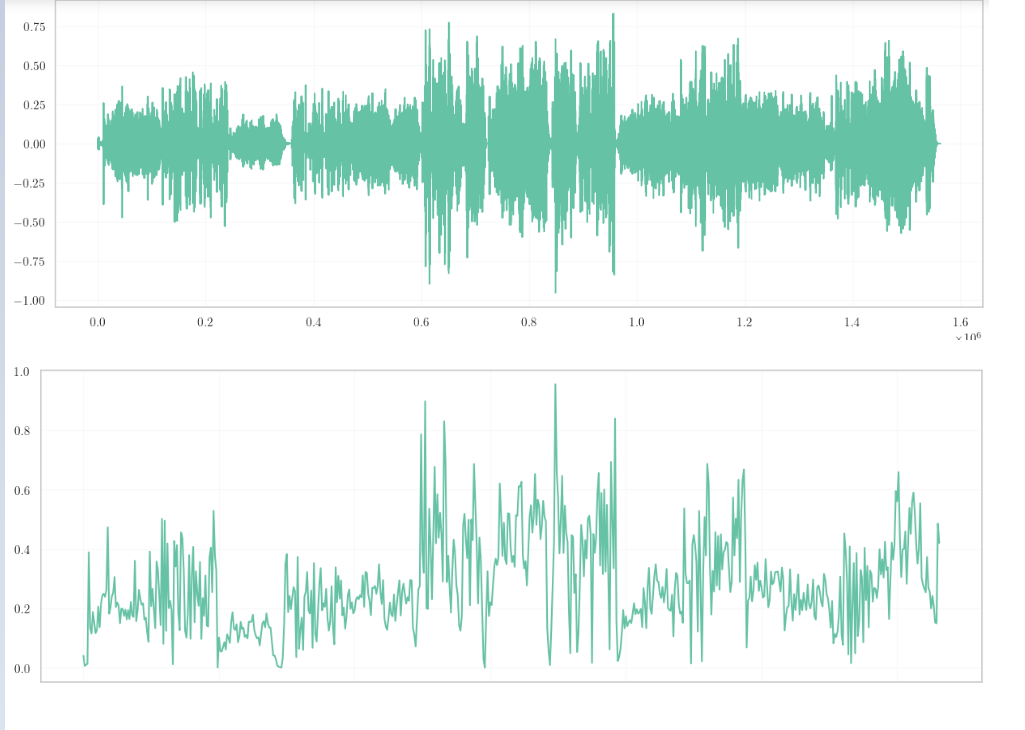
\includegraphics[width=1\textwidth]{granger.png}}
	\caption{Воксель, который предположительно зависит от звукового ряда}
	\label{fig:voxel}
\end{figure}


Оценим ошибку на этих вокселях, так как остальная часть не является следствием по Грэнджеру. Наименьшая скорректированная MSE достигается при задержке 4-5 секунд, что согласуется с данными, указанными в датасете.

\begin{figure}[h!]
	\centering{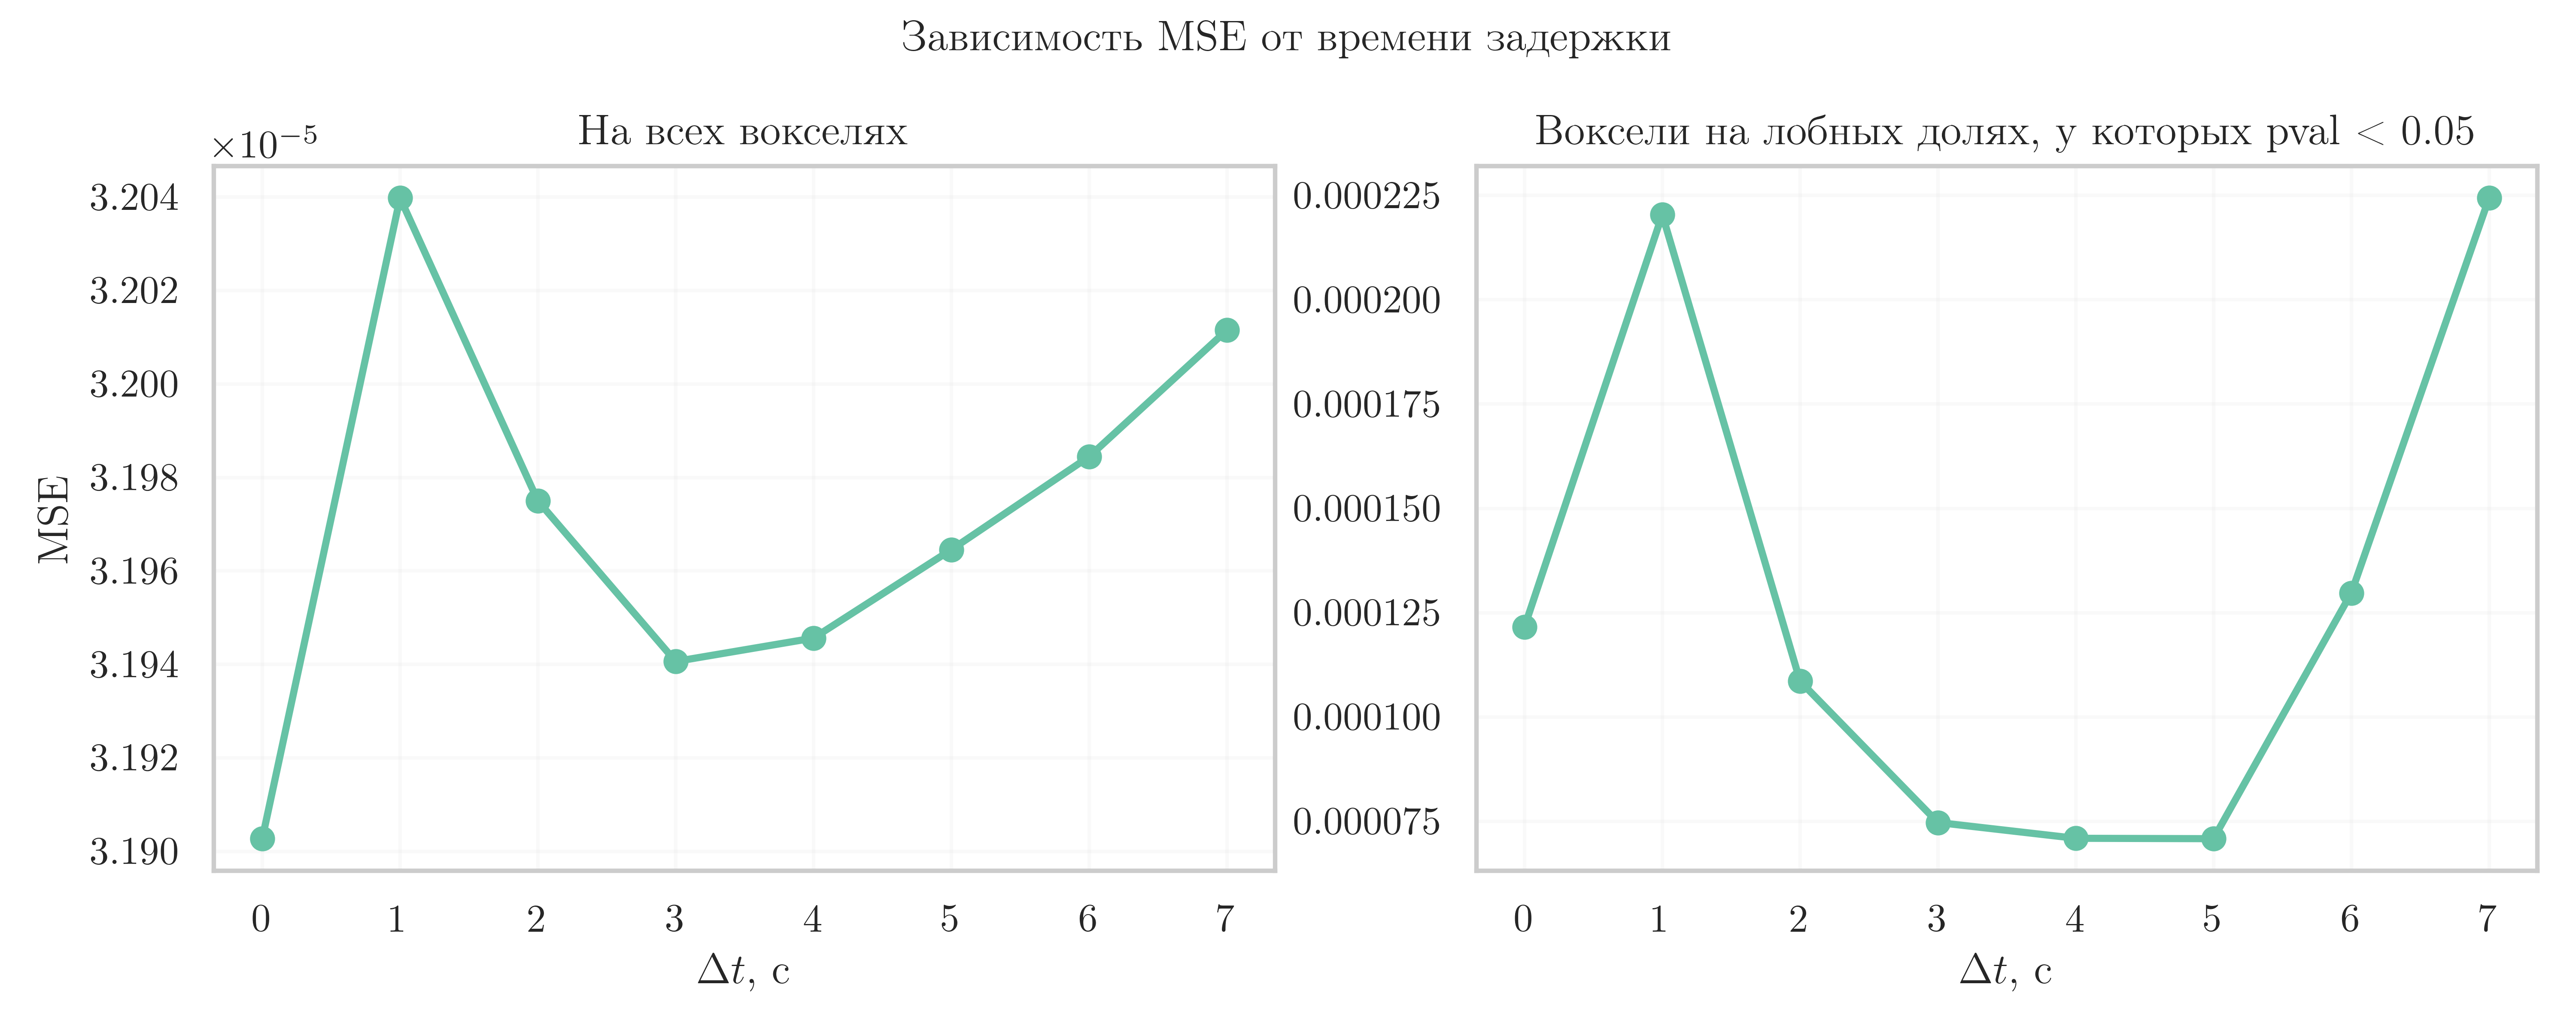
\includegraphics[width=1\textwidth]{mse_dt.png}}
	\caption{Скорректированный MSE}
	\label{fig:loc}
\end{figure}

\section{Заключение}
В данной работе рассматривается задача восстановления зависимости между показаниями фМРТ и звуковым рядом. Предложен метод аппроксимации последовательности фМРТ снимков с помощью звукового ряда. Метод учитывает временное разрешение снимков. Линейная модель строится независимо для каждого вокселя изображения фМРТ. Каждая линейная модель строится в предположении, что последовательность изображений фМРТ является марковской. Предложенная модель работает лучше чем неинформативная модель. Следовательно, звуковая дорожка влияет на изменения вокселей. Распределения весов модели невырожденные. Корректировка на воксели, которые предположительно являются следствием по Грэнджеру, уменьшают шум и MSE согласуется с временным разрешением в 4-5 секунд для испытуемого.
%%%% если имеется doi цитируемого источника, необходимо его указать, см. пример в \bibitem{article}
%%%% DOI публикации, зарегистрированной в системе Crossref, можно получить по адресу http://www.crossref.org/guestquery/
\renewcommand{\refname}{Литература}
\makeatletter
\renewcommand{\bibsection}{%
   \section{\refname%
            \@mkboth{\MakeUppercase{\refname}}{\MakeUppercase{\refname}}%
   }
}
\bibliographystyle{plain}
\bibliography{references.bib}

\end{document}
